\documentclass[10pt]{article} 
\usepackage[utf8]{inputenc}

%%% PAGE DIMENSIONS
\usepackage{geometry} 
\geometry{a4paper} 
\geometry{margin=.75in} 

%%% PACKAGES
\usepackage{booktabs} 
\usepackage{array} 
\usepackage{paralist}
\usepackage{verbatim} 
\usepackage{subfig} 
\usepackage{caption}
\usepackage{amsmath}
\usepackage{float}
\usepackage{color}
\usepackage[pdftex]{graphicx}

%%% HEADERS & FOOTERS
\usepackage{fancyhdr}
\pagestyle{fancy}
\renewcommand{\headrulewidth}{0pt}
\lhead{}\chead{}\rhead{}
\lfoot{}\cfoot{\thepage}\rfoot{}

%%% SECTION TITLE APPEARANCE
\usepackage{sectsty}
\allsectionsfont{\sffamily\mdseries\upshape}


%%% ToC (table of contents) APPEARANCE
\usepackage[nottoc,notlof,notlot]{tocbibind} 
\usepackage[titles,subfigure]{tocloft} 
\renewcommand{\cftsecfont}{\rmfamily\mdseries\upshape}
\renewcommand{\cftsecpagefont}{\rmfamily\mdseries\upshape} 

\title{Molecular Dynamics: Argon Gas Simulation}
\author{Mark Wittekind \& Drew Murray}

%\date{} % Remove the '%' before '\date{}' to display a given date or no date (if empty),
         % otherwise leave the '%' and the current date is printed 


\newcommand{\beq}{\begin{equation}} 
\newcommand{\eeq}{\end{equation}} 
\newcommand{\n}{\noindent} 


\begin{document}

\maketitle
\section{Introduction}
Simulating gas is, at best, an O($n^2$) operation as one must calculate force between each pair of particles every timestep.  This computational difficulty lends itself to a series of interesting and useful approximations which we explored in this project.  Our simulation can be broken into three main components:
\newline
\newline
1. Initial conditions of particles. \newline
2. Runtime calculations.\newline
3. Data collection and interpretation.\newline

	
In adjusting our initial conditions we can simulate different states of our particle collection, e.g. solid, liquid, or gas.  We can also observe the relationship between various observables, e.g. temperature, pressure, and energy.

\section{Initial Conditions}
\subsection{Lennard-Jones Potential}
\beq
\label{eqn:equation1}
 V(r) = 4\epsilon[(\sigma / r)^{12} -(\sigma / r)^6]
\eeq
The Lennard-Jones Potential, when minimized, yields the nearest distance between adjacent Argon atoms in a stable crystal lattice.  We utilize this minimum distance when initializing the positions of our particles.  From this we can derive the force on a particle:

\beq
\label{eqn:equation2}
F(r) = \epsilon[48{ \sigma ^{12} \over r^{13}} - 24{\sigma ^{6} \over r^{7}} ]
\eeq

\subsection{Position}
In utilizing the minimum of the Lennard-Jones Potential and arranging our particles into an FCC lattice we are initializing them in an arrangement near the ground state.
\newline
\newline
\beq
\label{eqn:equation3}
\frac{d}{dr}V(r) = -24\epsilon[2(\frac{\sigma^{12}}{r^{13}})-(\frac{\sigma^{6}}{r^{7}})] = 0
\eeq
\newline

The first image is of the unit cell.  The unit cell is the smallest repeating structure of the lattice and is made up of 4 base vectors.  The lattice is created by translating the base vectors in integer multiples of the width of the unit cell.  Such a lattice can be seen in figure 2.

\begin{figure}[ht]
\centering
\begin{minipage}{.45\textwidth}
\centering
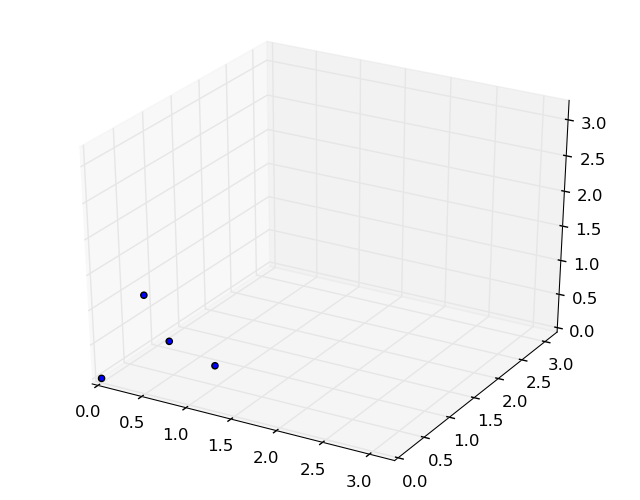
\includegraphics[width=0.5 \linewidth]{figures/Initial4.png}
\caption{Visual representation of base vectors (n = 4)}
\label{fig:figure1}
\end{minipage}\hfill
\quad	
\begin{minipage}{.45\textwidth}
\centering
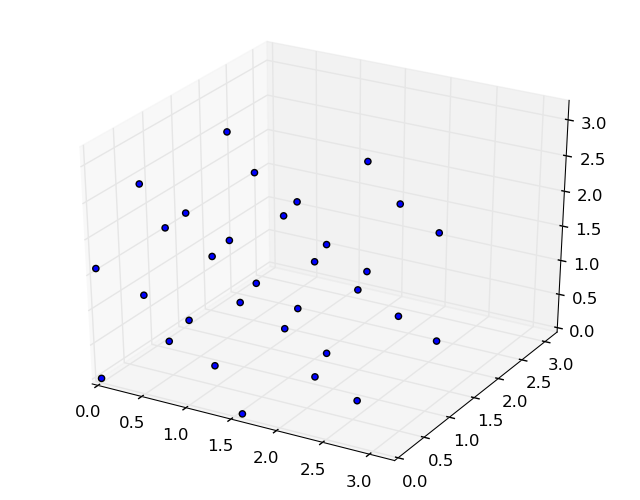
\includegraphics[width=0.5 \linewidth]{figures/Initial32.png}
\caption{Example of initial lattice (n = 32)}
\label{fig:figure2}
\end{minipage}\hfill
\end{figure}
\n

To simulate an infinite lattice, we employed periodic boundary conditions.  When a particle moved beyond the edge of our simulation-space, we replaced it on the other side.

\subsection{Velocity}
Our initial velocities follow a Gaussian distribution described by the Maxwell-Boltzmann distribution which is as follows:

\beq
\label{eqn:equation4}
Probability(E) \propto e^{-E/T}
\eeq
\newline
We must ensure the distribution is centered on zero to avoid drifting.  Further, we must re-scale the initial velocities so that our simulation starts off at a desired temperature.  This procedure is also useful later as a thermostat to ensure our system maintains a particular temperature.


\section{Runtime}
\subsection{Numerical Integration in Time}
The Verlet algorithm lends itself to the ratio of accuracy and performance that we require (O($n^2$)).  It works by using half timesteps by calculating the intial velocity, updating to one half timestep later, re-calculating velocity, and finishing the timestep.  Mathematically the result is as follows:

\beq
\label{eqn:equation5}
\textbf{r}(t+dt) = \textbf{r}(t) + dt\textbf{v}(t) + dt^2\textbf{F}(t)/2
\eeq

\beq
\label{eqn:equation6}
\textbf{v}(t+dt) = \textbf{v}(t) + dt[\textbf{F}(t+h)+\textbf{F}(t)]/2
\eeq
\newline

\subsection{Computational Limitations}
The Verlet algorithm depends on calculating the net force on each particle twice per timestep, in three dimensions.  Each particle feels a force from every other particle.  Therefore finding the force requires a calculation proportional to the number of possible pair combinations of particles ($n^2$).  Running the simulation for a sufficient number of timesteps with a large number of particles is a major obstacle.
In addition, each particle's position, velocity, and acceleration in each of three dimensions must be stored.  This means that the memory usage is at best $O(9n)$.  If the particles positions are recorded at multiple intervals throughout the simulation, then the memory requirements can become prohibitive.

\subsection{Thermostat}
Using the relationship between temperature and the expectation value of velocity squared we derived a scaling factor:

\beq
\label{eqn:equation7}
\lambda = \sqrt{\frac{3k_BT_{0}}{m<v_{cur}^2>}}
\eeq
\newline

where $T_{0}$ is the desired temperature and $v_{cur}$ is the current velocity.

We can use this scaling factor to re-adjust the temperature of our gas throughout the simulation.  

\section{Observations \& Measurements}
We expect the following relationships for observables:

	\begin{center}
	$Pressure \propto Temperature \propto Kinetic Energy$
	\end{center}
	
	\begin{center}
	$d(Kinetic Energy) = -d(Potential Energy)$
	\end{center}
	

\subsection{Energy Conservation}
For an accurate simulation we must ensure energy is conserved.  We can find the total energy by summing the potential and kinetic components which are found as follows:

\beq
\label{eqn:equation8}
E_K = \frac{1}{2}m(\textbf{v}_{i}\cdot\textbf{v}_j)
\eeq
\beq
\label{eqn:equation9}
E_P = 4\epsilon[(\frac{2\sigma}{\textbf{r}_{i-j}\cdot\textbf{r}_{i-j}})^6-(\frac{2\sigma}{\textbf{r}_{i-j}\cdot\textbf{r}_{i-j}})^3]
\eeq

Our energy is, as shown below, is constant despite our injections of kinetic energy through our thermostat.  Also shown is a plot of energy when initialized at T=0; the rapid fluctuations about zero are due to rounding errors.  The result around T=0 suggests our lattice is sufficiently symmetric to maintain the initial structure and thus our boundary conditions are working and balancing the forces between particles.

\begin{figure}[ht]
\centering
\begin{minipage}{.45\textwidth}
\centering
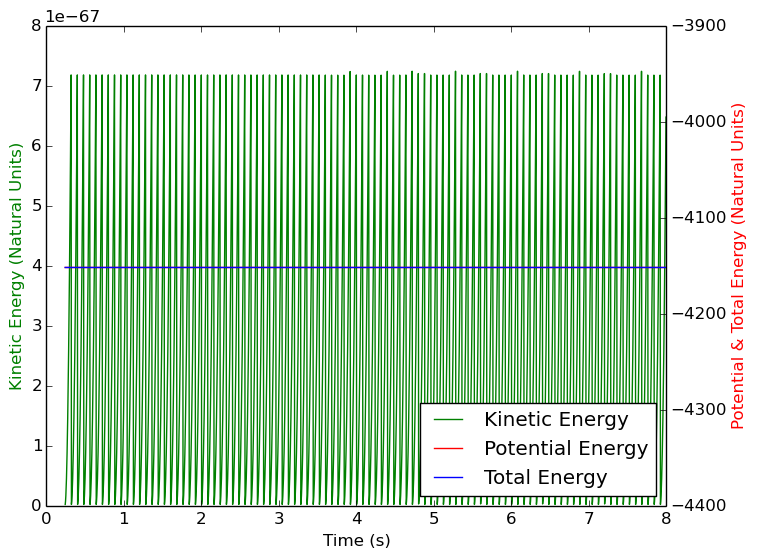
\includegraphics[width=1 \linewidth]{figures/energy0.png}
\caption{Energy around T=0}
\label{fig:figure3}
\end{minipage}\hfill
\quad	
\begin{minipage}{.45\textwidth}
\centering
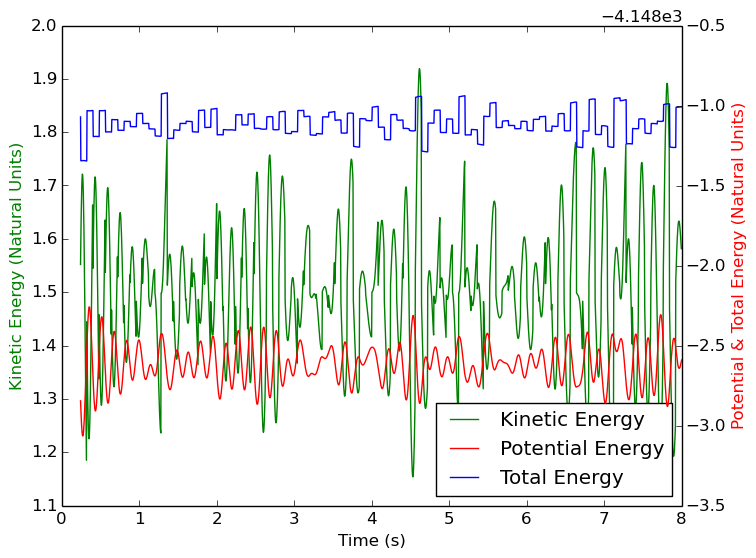
\includegraphics[width=1 \linewidth]{figures/energy1.png}
\caption{Energy around T=1}
\label{fig:figure4}
\end{minipage}\hfill
\end{figure}
\n
\begin{figure}[ht]
\centering
\begin{minipage}{.45\textwidth}
\centering
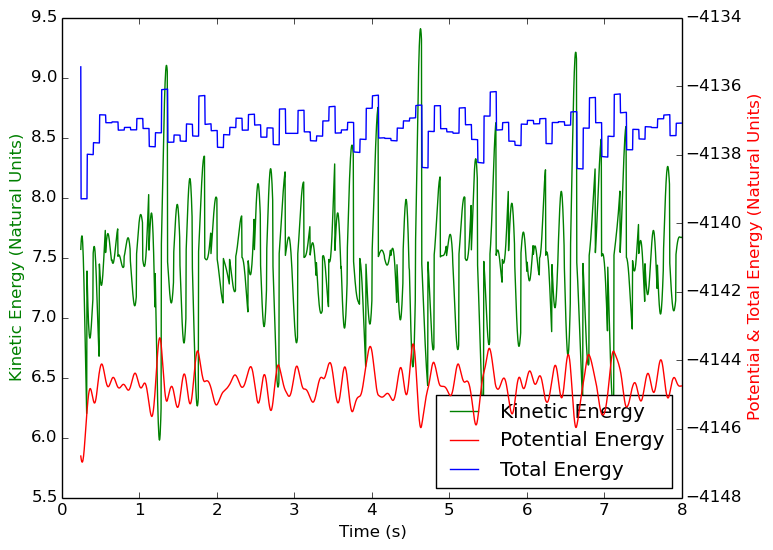
\includegraphics[width=1 \linewidth]{figures/energy2.png}
\caption{Energy around T=5}
\label{fig:figure4}
\end{minipage}\hfill
\end{figure}

\subsection{Temperature}
Our thermostat is used to maintain temperature in our simulation so we can explore properties at particular temperatures.  We calculate the temperature of our system as follows:

\beq
\label{eqn:equation10}
T = \frac{2K_E}{2k_B}
\eeq

\begin{figure}[H]
\centering
\begin{minipage}{.45\textwidth}
\centering
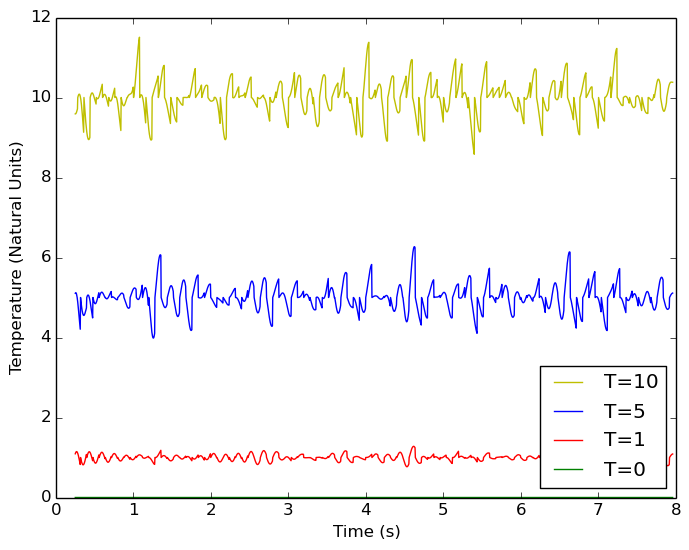
\includegraphics[width=1 \linewidth]{figures/temp.png}
\caption{Temperature around T=(10,5,1,0)}
\label{fig:figure5}
\end{minipage}\hfill
\end{figure}

\subsection{Pressure}
Because volume, number of particles, and temperature are maintained we expect pressure to be maintained and remain strongly correlated to temperature.  This behavior is similar to that of an ideal gas with a small correction factor.  We calculate pressure as follows: 

\beq
\label{eqn:equation11}
P = k_BT + \frac{1}{3n}<\sum\limits_{i}^n\sum\limits_{j>i}^n\textbf{r}_{ij}\textbf{F}_{ij}>
\eeq

\begin{figure}[ht]
\centering
\begin{minipage}{.45\textwidth}
\centering
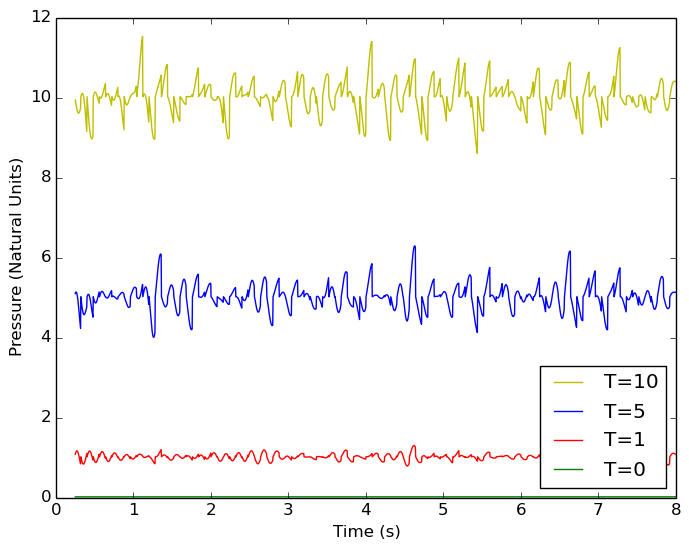
\includegraphics[width=1 \linewidth]{figures/pressure.png}
\caption{Pressure around T=(10,5,1,0)}
\label{fig:figure6}
\end{minipage}\hfill
\end{figure}

\subsection{Pair Correlation}
As the temperature of the crystal increases, the atoms begin to move away from their starting positions.  The distances between the atoms shifts from being integer multiples of the minimum distance ($\sigma$) to being more random.  In the liquid and gaseous state there is no observable pattern to the distribution of the distances.
Figure 7 shows the strong peaks at the integer multiples of $\sigma$.  Figure 8 shows some smoothing of the peaks: the particles are near their starting positions, but are allowed to move around.  Figure 9 shows the complete lack of correlation between the positions and the lattice.  This means that the particles are moving and positioned randomly. 

\beq
\label{eqn:equation12}
bin_k = \frac{1}{N(N-1)dV}\sum\limits_{i}^n\sum\limits_{j>i}^nr_k<r_{ij}<(r_{k}+dr)
\eeq

where:

\beq
\label{eqn:equation13}
dV = \frac{4\pi}{3}[(r_k+dr)^3-(r_k)^3]
\eeq

\begin{figure}[H]
\centering
\begin{minipage}{.45\textwidth}
\centering
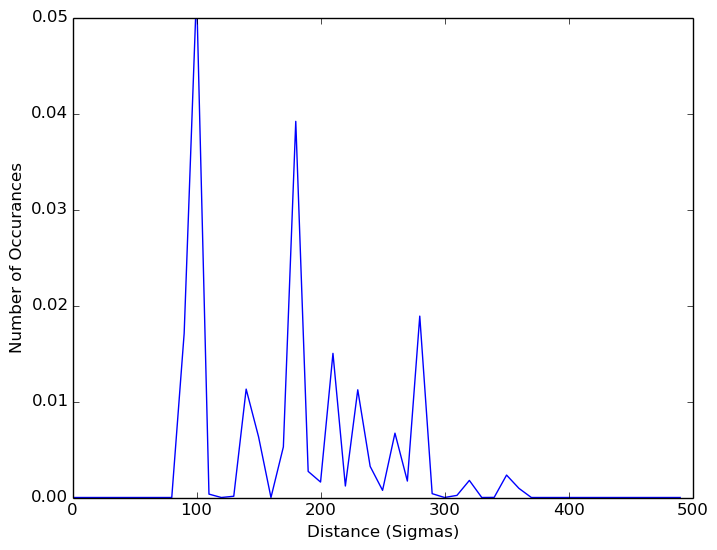
\includegraphics[width=1 \linewidth]{figures/correlation0.png}
\caption{Pair correlation around T=0 showing the strong peaks at integer multiples of $\sigma$.}
\label{fig:figure7}
\end{minipage}\hfill
\quad	
\begin{minipage}{.45\textwidth}
\centering
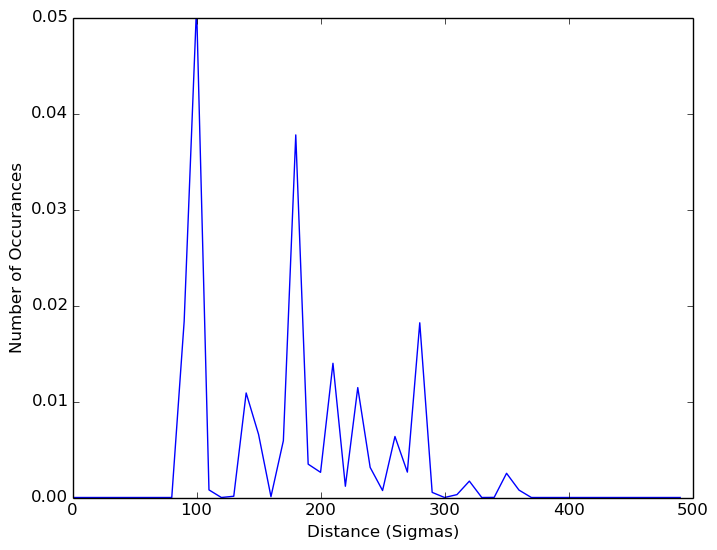
\includegraphics[width=1 \linewidth]{figures/correlation2.png}
\caption{Pair correlation around T=1 showing the weaker, yet distinct, peaks at integer multiples of $\sigma$.}
\label{fig:figure8}
\end{minipage}\hfill
\end{figure}
\n
\begin{figure}[H]
\centering
\begin{minipage}{.45\textwidth}
\centering
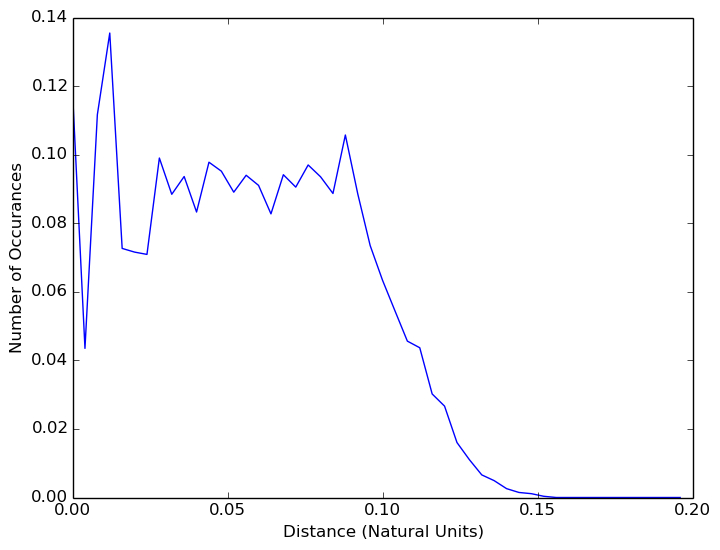
\includegraphics[width=1 \linewidth]{figures/correlation10.png}
\caption{Pair correlation around T=10 showing a nearly random distribution.}
\label{fig:figure9}
\end{minipage}\hfill
\end{figure}

\section{Conclusion}

By simulating the Lennard-Jones interactions between particles we can measure the relationships between observables at the temperatures near the critical point of phase transition.  We modeled Argon's transition from a solid to a liquid and then a gas.  By utilizing periodic boundary conditions we successfully simulated an infinite arrangement of particles at different temperatures.  We demonstrated the expected relations between energy, pressure, temperature, and spacial correlation.

	



\end{document}